% $Id : latex . tex 179 2016 -03 -01  D guzman $
%Document configuration
\documentclass [12 pt , a4paper ] {article}
\setlength {\topmargin }{ -2 cm }
\setlength {\oddsidemargin }{0 cm }
\setlength {\textheight }{24 cm }
\setlength {\textwidth }{16 cm }
%General format packages
\usepackage[utf8]{inputenc}
\usepackage[english]{babel}
%Graphics package
\usepackage {graphicx}
%Graphics configuration
\graphicspath{ {images/} }
\DeclareGraphicsExtensions{.png}
%Bibliography
\usepackage[backend=biber]{biblatex}
%Additional package for babel package required by biblatex
\usepackage{csquotes}
%Bibliography config
\addbibresource{bibliography.bib}
%package to include pieces of code
\usepackage{listings}

%start document
\begin{document}
\title{\huge \textbf { Homework 2: Tools of the Trade - Statistics}}
\date { November, 9th 2016 }
%\author { David Guzm\'an }
\author { No Group - David Guzm\'an }
\maketitle
\tableofcontents{}
\newpage
%%%%%%%%%%%%%%%%%%%%%%%%%%%%%%%%%%%%%%%%%%%%%%%%%%%%%%%%%%%%%%%%%%%%%%%%%%%%%%%%%%%
\section{Computing variables and checking assumptions}
\subsection{What is the ECDF F (x) of the data set?}
\par Data set: $[ -10.1,-1.2,-9.5,-1,-1,-1,0.1, 5, 7, 7, 7, 7, 2, 2, 2 ]$ .
\begin{figure}[!ht]
  \centering
  \includegraphics[scale=0.2,width=0.75\textwidth, natwidth=7000,natheight=1000]{ecdf.eps}
  \caption{Dataset}
  \label{fig:Dataset}
\end{figure}
\par The ECDF defined as $F(x)= \frac{1}{n} \sum\limits_{n=1}^{n} 1_{\{x_i\leq x\}}$.
\\ For the case: $x=-100$, we get $F(-100)= \frac{1}{n} \sum\limits_{n=1}^{n} 1_{\{x_i\leq-100\}} = 0$
\\ For the case: $x=-10$, we get $F(-10)= \frac{1}{n} \sum\limits_{n=1}^{n} 1_{\{x_i\leq-10\}} = 1/15$
\\ For the case: $x=0$, we get $F(0)= \frac{1}{n} \sum\limits_{n=1}^{n} 1_{\{x_i\leq0\}} = 6/15$
\\ For the case: $x=7$, we get $F(7)= \frac{1}{n} \sum\limits_{n=1}^{n} 1_{\{x_i\leq7\}} = 1$
\\ For the case: $x=10$, we get $F(10)= \frac{1}{n} \sum\limits_{n=1}^{n} 1_{\{x_i\leq10\}} = 1$
\subsection{ What is the median?}
\par The median defined as $x_{(\frac{n}{2})}$ iff $n$ is odd and $\frac{1}{2}(x_{(\frac{n}{2})} + x_{(\frac{n}{2}+1)})$ for the rest \cite{leboudec}.
\\ Let $xi<xj$ if $i<j$
\\ Median of: $x_{-2}, x_1,x_0$ is equal to: $x_0$
\\ Median of: $x_{-2}, x_1,x_0,x_2,x_4,x_{-3}$ is equal to: $\frac{x_0+x_1}{2}$
\\ Median of: $ [-10.1, -9.5, -1.2, -1, -1, -1, 0.1, 2, 2, 2, 5, 7, 7, 7, 7] $ is equal to: $2$
\subsection{What is the main necessary assumption for the calculation of a confidence interval?}
\par We assume that the data is coming from an
Independent Identically Distributed stochastic model (random variables) \cite{leboudec}.
\subsection{Compute the confidence interval for the median}
\par Dataset: $ [-10.1, -9.5, -1.2, -1, -1, -1, 0.1, 2, 2, 2, 5, 7, 7, 7, 7] $
\par Using the tables \cite{leboudec} to determine confidence intervals
for quantiles (including the median), according to Theorem Confidence Interval for the Median and other Quantiles.
For a sample of n \emph{iid} data points $x_1,...,x_n$,
the tables give a confidence interval at the confidence level $\lambda = 0.95$ or $ \lambda=0.99$
for the q-quantile with $q = 0.5$ (median) \cite{leboudec}.
\par For the sample Dataset: $n=10$ and median $m = x_{(8)} = 2$, and using apendix A from \cite{leboudec}
we get for $n=15$, $j=4$, $k=12$ and $p=0.965$, the confidence interval given by the Figure~\ref{fig:confidenceintervals}
is $[x_{(4)}=-1, x_{(12)}=7]$, as we can observe in Figure~\ref{fig:boxplot}.
\begin{figure}[!ht]
  \centering
  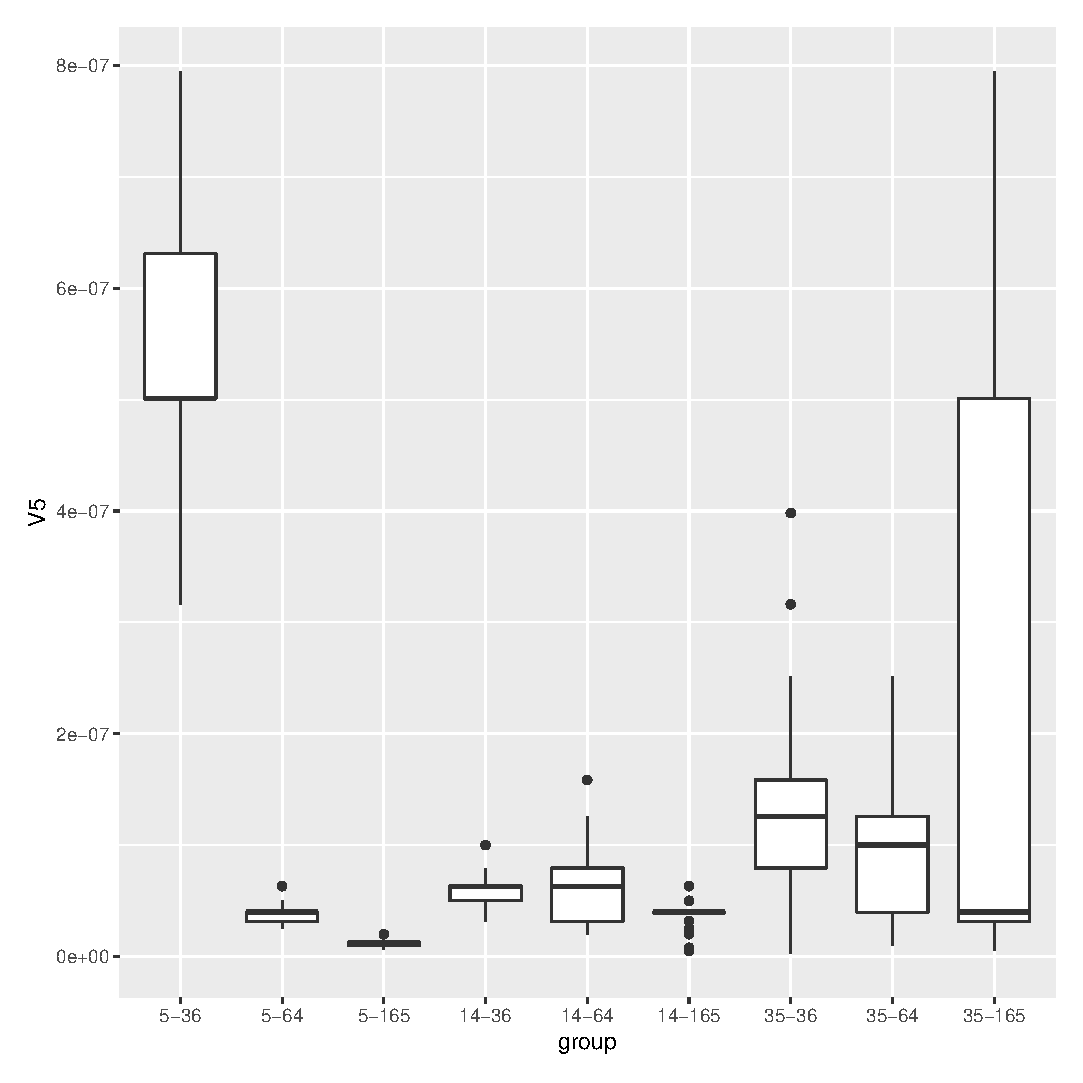
\includegraphics[scale=0.2,width=0.45\textwidth, natwidth=7000,natheight=1000]{boxplot.eps}
  \caption{Box Plot Confidence Intervals}
  \label{fig:boxplot}
\end{figure}
\begin{figure}[!ht]
  \centering
  \includegraphics[scale=0.2,width=0.75\textwidth, natwidth=7000,natheight=1000]{1.png}
  \caption{Confidence Intervals \cite{leboudec}}
  \label{fig:confidenceintervals}
\end{figure}
\subsection{Does it make sense to compute a confidence interval for the mean on the data set in (a)? Why (not)?}
\par The mean $m$ of a data set $x_1,...,x_n$
is $m = \frac{1}{n} \sum\limits_{i=1}^{n} x_i $, and gives
information about the average \cite{leboudec}, for
this case $m=1.02$. Even though, the assumptions, data source is coming from iid, large number
of samples, and it is a common distribution with a finite
variance, and for $n<30$ data must come from \emph{iid} and a \emph{normal distribution}
are strictly neccesary, \emph{the computation of a confidence interval
for the mean does make sense, for it characterizes both the variability
of the data and the accuracy of the measured average} \cite{leboudec}. Although,
we can inspect in Figure~\ref{fig:qqplot} , which shows  the quantiles of the
measurements against the corresponding
quantiles of the normal distribution,
 data is not coming from a normal distribution. As a result,
 we should re-scale through for example Box-Cox transformation
 to compute a better approach to the CI for mean\cite{leboudec}.
\begin{figure}[!ht]
  \centering
  \includegraphics[scale=0.2,width=0.55\textwidth, natwidth=7000,natheight=1000]{qqplot.eps}
  \caption{QQPlot Normal Distribution for Data Set [x]}
  \label{fig:qqplot}
\end{figure}

 \subsection{If the confidence interval of the difference between the means of two data
 sets includes 0, what does it imply? }
 \par When we claim that an interval $I$ is a confidence interval
 at the level $0.95$ for a certain parameter $\theta$, we mean the following.
 Repeating the experiment many times would lead to,
 in about $95\%$ of the cases, the interval $I$ indeed containing
 the true value $\theta$ \cite{leboudec}. Hence, if a confident interval for a mean
 difference \emph{includes} $0$, \emph{the data set is consistent with another
  data set (population) mean difference of $0$} \cite{jerry}.
 \subsection{What is the simple moving average of the data set in (a) with n = 3?}
 \par For SMA defined as: $SMA = \frac{1}{n} \sum\limits_{i=0}^{n-1} p_{(M-i)} $
 \\ for $n=3$ : $SMA = \frac{1}{3} \sum\limits_{i=0}^{3-1} p_{(M-i)} = -6.93, -1,4.03,7,2 $
 \section{Reading a plot}
 \par The following plot shows the result of a performance test over two different wireless links:
 \begin{figure}[!ht]
   \centering
   \includegraphics[scale=0.2,width=0.75\textwidth, natwidth=7000,natheight=1000]{2.png}
   \caption{Throughput}
   \label{fig:throughput}
 \end{figure}

 \subsection{What is the metric here?}
 \par Throughput
 \subsection{What are the median, the quartiles and the $95\%$ quantiles for both links?}
\par According to Figure~\ref{fig:throughput}:
 \par Median Link A = $5Mbps$, Median Link B = $6Mbps$
 \par $25\%$ Quartil Link A = $4.8Mbps$, $25\%$ Quartil Link B = $5.2Mbps$
 \par $75\%$ Quartil Link A = $5.3Mbps$, $75\%$ Quartil Link B = $7Mbps$
 \par $95\%$ Quantil Link A = $5.8Mbps$, $95\%$ Quantil Link B = $8Mbps$
 \par $5\%$ Quantil Link A = $4.3Mbps$, $5\%$ Quantil Link B = $4.3Mbps$
 \subsection{Which link do you think has the higher mean? Which one has the higher standard deviation? Why?}
 \par Link B has the higher mean because the measurements in the
 different quartiles and quantiles
 are always higher, and due to the fact that the balance point for the area
 under the curve for Link B is higher (between 7 and 9) than the balance point for Link A (bet
 ween 4 and 6).
 \subsection{Based on this data, which link do you think had the better performance? Why?}
 \par Link B, measurements of throughput are higher than Link A.
 \subsection{What possible factors could have influenced the performance?}
\par Range between the two points establishing the communication measured (Proximity to AP),
we could reference the Figure~\ref{fig:wifi}, to have an idea of the rate variation
according to the distance for the IEEE 802.11 standard.
\begin{figure}[!ht]
  \centering
  \includegraphics[scale=0.2,width=0.35\textwidth, natwidth=7000,natheight=1000]{3.png}
  \caption{802.11 Data Rate \cite{langar}}
  \label{fig:wifi}
\end{figure}
\par Receiving Sensivity in the client card that could affect the EIRP(Effective
Isotropic Radiated Power \cite{schiller}) in the total link budget, as we could infer from
Figure~\ref{fig:sensitivity}.
\begin{figure}[!ht]
  \centering
  \includegraphics[scale=0.2,width=0.35\textwidth, natwidth=7000,natheight=1000]{4.png}
  \caption{Sensitivity in Cards \cite{schiller}}
  \label{fig:sensitivity}
\end{figure}
\par Noise and weather affecting free space propagation.
\par Change in antennas gain configuration.
\par Different Coding Schemes according to the version of the protocol, for example 802.11b
systems offer 11, 5.5, 2 ,or 1 Mbps, with maximun user data rate approx 6Mbps. The
lower data rates use DBPSK or DQPSK \cite{schiller}.
\begin{figure}[!ht]
  \centering
  \includegraphics[scale=0.2,width=0.45\textwidth, natwidth=7000,natheight=1000]{5.png}
  \caption{Rate Dependent Parameters for IEEE 802.11a \cite{schiller}}
  \label{fig:sensitivity}
\end{figure}

  % \par Figure \ref{fig:80211Frame} shows the basic structure of an IEEE 802.11 MAC data frame
  % together with the contect of the frame control field \cite{schiller}, where Frame Control are the
  % first two bytes serve several purposes, like fragmentation, retransmission, power management
  % , and security negotiation.

%Prints the bibliography
\printbibliography
\end{document}
